% nladoc.tex V2.0, 13 May 2010

\RequirePackage{fix-cm}
\documentclass[smallcondensed,final]{svjour3}     % onecolumn (ditto)

\usepackage{moreverb}

\usepackage[colorlinks,bookmarksopen,bookmarksnumbered,citecolor=red,urlcolor=red]{hyperref}
\usepackage{tikz}
\usetikzlibrary{shapes,arrows,trees,snakes} %,decorations.pathreplacing,fit}
% \usepackage{tkz-euclide}
\usepackage{pgfplots}
\usepackage{caption,subcaption}
% \usetkzobj{all} 
\usepackage{amsmath}

\definecolor{utorange}{RGB}{203,96,21}
\definecolor{utblack}{RGB}{99,102,106}
\definecolor{utbrown}{RGB}{110,98,89}
\definecolor{utsecbrown}{RGB}{217,200,158}
\definecolor{utsecgreen}{RGB}{208,222,187}
\definecolor{utsecblue}{RGB}{127,169,174}


\newcommand{\todo}[1]{\textcolor{red}{\bf #1}}
\newcommand{\gsnote}[1]{\textcolor{blue}{GS: #1}}


\newcommand\BibTeX{{\rmfamily B\kern-.05em \textsc{i\kern-.025em b}\kern-.08em
T\kern-.1667em\lower.7ex\hbox{E}\kern-.125emX}}

%\def\volumeyear{2013}

\begin{document}

\titlerunning{High-order Geometric Multigrid Methods}

\title{Comparison of Geometric Multigrid Algorithms for High-order Finite Element Discretizations}

\author{Hari Sundar, Georg Stadler, Omar Ghattas and George Biros}

\institute{Institute for Computational Engineering \& Sciences, The
  University of Texas at Austin, Austin, TX}

%\corraddr{\texttt{hari@ices.utexas.edu}}
\maketitle

\begin{abstract}
We are interested in asymptotically
optimal---$\mathcal{O}(N)$---complexity solvers for approximating the
solution of elliptic partial differential equations (PDEs), where $N$
is the number of unknowns.  Multigrid is such a solver. In practice
however, multigrid performs best for low-order uniform discretizations
with smooth coefficients.
%
Our goal is to compare different geometric multigrid approaches for
solving systems arising from high order discretizations of
variable-coefficient elliptic partial differential equations on
arbitrary geometries. High order discretizations offer several
advantages over low-order discretizations. Besides the faster
convergence per unknown for sufficiently smooth problems, high order
discretizations can often make better use of modern hardware due to
their locality, resulting in improved efficiency of the calculations.
%  According to standard isoparametric polynomial
%approximation theory, by using a finite element basis of at least
%degree $p$, we can achieve very fast $\mathcal{O}(N^{-(p+1)})$
%convergence for sufficiently smooth problems while improving the
%locality and thus the CPU efficiency of the calculations.
\end{abstract}

\keywords{geometric multigrid, high order finite elements, p-multigrid}



\section{Introduction}

This paper presents a systematic comparision of geometric multigrid
algorithms for the solution of systems arising from high order (we
target polynomial orders up to 16) discretizations of elliptic partial
differential equations. Our particular interest is to compare the
efficiency of different high order multigrid methods for problems with
varying coefficients and complex geometry.

While we use moderate size model problems for the comparisons in this
paper, we also discuss our findings with regard to parallel
implementations on high performance computing platforms.  In
particular, we discuss (1) matrix-free methods, i.e., methods that do
not require assembled finite element matrices, and (2) their
parallelization on shared or distributed memory architectures.
% and (3)
% cache-efficient methods with dominantly local memory access.

High order spatial discretizations can have significant advantages
over low order methods, especially when the solution is smooth and
high accuracy is desired. However, the sparsity of finite element (or
finite difference) operators decreases as the polynomial approximation
order increases, which makes the application of high order operators
to vectors computationally significantly more expensive. This is also
true if matrix-free methods are used, i.e., system matrices are never
assembled, but their application on vectors is implemented through
elemental loops.  Besides the loss of sparsity, another challenge in
high order discretizations is due to the fact that the discretization
matrices loose structural properties such as the M-matrix property,
which allows to prove convergence of iterative solvers such as the
Jacobi or Gauss-Seidel method.

\noindent
\gsnote{Needs a literature review.}\\

\begin{itemize}

\item Large-scale simulations, target:
\cite{SundarBirosBursteddeEtAl12}

\item Direct application of AMG to high order systems:
\cite{HeysManteuffelMcCormickEtAl05}

\item Low-order preconditioning of high order systems:
\cite{Brown10,Kim07,DevilleMund90,HeysManteuffelMcCormickEtAl05}.

\end{itemize}

\noindent
%\gsnote{Unify notion of mesh/grid etc}\\
% \gsnote{Unify use of high order vs.\ higher order}\\
\gsnote{We use hexas, motivated from spectral methods. Main
  advantage is tensorized basis functions (and, potential octree adaptivity)}\\
\gsnote{High order discretizations map better to current architectures}


For three-dimensional hexahedral mesh finite element discretizations
with polynomial degree $p$, element matrices are of size
$n=(p+1)^3$. The naive assembly and application of these elemental
matrices requires $\mathcal O(p^9)$ operatrions, but exploiting the
tensor structure of the basis functions allows to reduce this to
$\mathcal O(p^7)$ operations.


Although there are examples of using Algebraic Multigrid directly on
operators resulting from high order discretizations, limited work
has been done on using geometric multigrid with high order
discretizations. To the best of our knowledge, no prior work on using
geometric multigrid for solving systems arising from high order
discretizations on arbitrary geometries using highly adapted meshes.



%In this work, we develop
%geometric multigrid methods to support higher-order discretizations
%($1\le p\le 8$) and compare  against preconditioning using the
%co-located linear operator.

% We evaluate using variable-coefficient
%Poisson problems on $2D$ and $3D$ domains. We demonstrate that by
%using appropriate inter-grid transfer operators and smoothers,
%mesh-independent convergence is possible ($1\le p\le8$) for the {\em
%direct} approach. For the direct approach, best results are obtained
%using the symmetric successive over-relaxation (SSOR) smoother. We
%conclude with thoughts on the parallelization of the proposed
%approach.\\[2ex]


%\section{Meshing, High-order FEM}


%Our method is designed for meshes that are built from an unstructured
%hexahedral macro mesh, in which each macro element is adaptively
%refined as an octree. This forest-of-octrees approach enables us to
%generate meshes for complex geometries with arbitrary levels of local
%refinement. We use geometric multigrid (GMG) for each of the octrees
%and algebraic multigrid (AMG) as the coarse grid solver. We designed
%our GMG sweeps to entirely avoid collectives, thus minimizing
%communication cost. Recently \cite{SundarBirosBursteddeEtAl12}, we
%presented weak and strong scaling results for the 3D
%variable-coefficient Poisson problem using linear discretization that
%demonstrate high parallel scalability. Here we explore various
%approaches for extending our geometric multigrid solver to support
%higher-order discretizations.


\section{Approaches for high order multigrid}
\label{sec:approaches}
% talk about the 4 main approaches and prior work.

In this section, we summarize different approaches to geometric
multigrid for high order finite element discretizations; for an
overview see Figure~\ref{fig:approaches}. These methods can either be
directly used as solvers, or as preconditioners within a Krylov method.

\begin{figure}
		% illustration for p-multigrid
		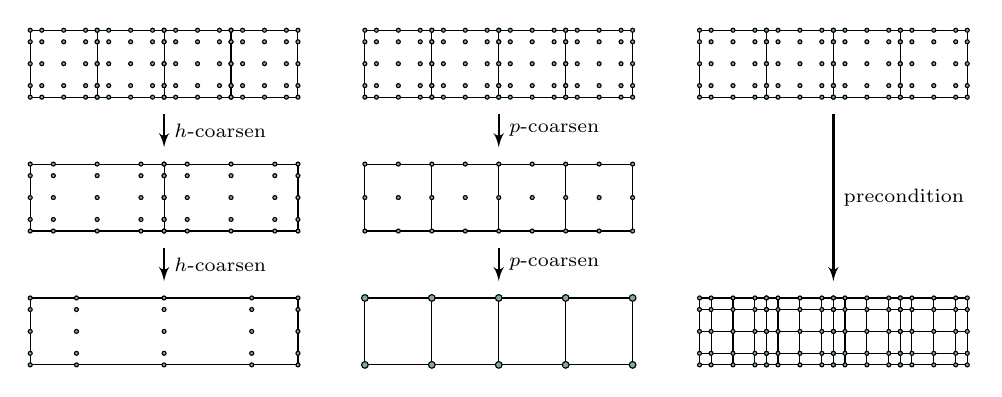
\begin{tikzpicture}[scale=0.85]
		% homg
		\draw (-5,4) grid +(4,1);
		\foreach \e in {-5,...,-2}
		\foreach \x in {0,0.1727,0.5,0.8273, 1.0} {
			\draw[fill=utsecblue] (\e+\x, 4) circle (0.03);
			\draw[fill=utsecblue] (\e+\x, 4.1727) circle (0.03);
			\draw[fill=utsecblue] (\e+\x, 4.5) circle (0.03);
			\draw[fill=utsecblue] (\e+\x, 4.8273) circle (0.03);
			\draw[fill=utsecblue] (\e+\x, 5) circle (0.03);
		}
		%\node at (5,4.5) {\small $p=4$};
		\draw[-latex',thick] (-3, 3.75) -- node[right] {{\scriptsize $h$-coarsen}} (-3, 3.25);
		\draw (-5,2) rectangle +(4,1);
		\draw (-3,2) -- (-3,3);
		\foreach \e in {-5,-3}
		\foreach \x in {0,0.1727,0.5,0.8273, 1.0} {
			\draw[fill=utsecblue] (\e+2*\x, 2) circle (0.03);
			\draw[fill=utsecblue] (\e+2*\x, 2.1727) circle (0.03);
			\draw[fill=utsecblue] (\e+2*\x, 2.5) circle (0.03);
			\draw[fill=utsecblue] (\e+2*\x, 2.8273) circle (0.03);
			\draw[fill=utsecblue] (\e+2*\x, 3) circle (0.03);
		}
		%\node at (5,2.5) {\small $p=2$};
	
		\draw[-latex',thick] (-3, 1.75) -- node[right] {{\scriptsize $h$-coarsen}} (-3, 1.25);
	
		\draw (-5,0) rectangle +(4,1);
		\foreach \x in {0,0.1727,0.5,0.8273, 1.0} {
			\draw[fill=utsecblue] (-5+4*\x, 0) circle (0.03);
			\draw[fill=utsecblue] (-5+4*\x, 0.1727) circle (0.03);
			\draw[fill=utsecblue] (-5+4*\x, 0.5) circle (0.03);
			\draw[fill=utsecblue] (-5+4*\x, 0.8273) circle (0.03);
			\draw[fill=utsecblue] (-5+4*\x, 1) circle (0.03);
		}
		
	%% p-multigrid
		\draw (0,4) grid +(4,1);
		\foreach \e in {0,...,3}
		\foreach \x in {0,0.1727,0.5,0.8273, 1.0} {
			\draw[fill=utsecblue] (\e+\x, 4) circle (0.03);
			\draw[fill=utsecblue] (\e+\x, 4.1727) circle (0.03);
			\draw[fill=utsecblue] (\e+\x, 4.5) circle (0.03);
			\draw[fill=utsecblue] (\e+\x, 4.8273) circle (0.03);
			\draw[fill=utsecblue] (\e+\x, 5) circle (0.03);
		}
		%\node at (5,4.5) {\small $p=4$};
	
		\draw[-latex',thick] (2, 3.75) -- node[right] {{\scriptsize $p$-coarsen}} (2, 3.25);
	
		\draw (0,2) grid +(4,1);
		\foreach \x in {0,0.5,...,4} {
			\draw[fill=utsecblue] (\x, 2) circle (0.03);
			\draw[fill=utsecblue] (\x, 2.5) circle (0.03);
			\draw[fill=utsecblue] (\x, 3) circle (0.03);
		}
		%\node at (5,2.5) {\small $p=2$};
	
		\draw[-latex',thick] (2, 1.75) -- node[right] {{\scriptsize $p$-coarsen}} (2, 1.25);
	
		\draw (0,0) grid +(4,1);
		\foreach \x in {0,1,2,3,4} {
			\draw[fill=utsecblue] (\x, 0) circle (0.05);
			\draw[fill=utsecblue] (\x, 1) circle (0.05);
		}
		%\node at (5,0.5) {\small $p=1$};
		
		%% collocated
			\draw (5,4) grid +(4,1);
			\foreach \e in {5,...,8}
			\foreach \x in {0,0.1727,0.5,0.8273, 1.0} {
				\draw[fill=utsecblue] (\e+\x, 4) circle (0.03);
				\draw[fill=utsecblue] (\e+\x, 4.1727) circle (0.03);
				\draw[fill=utsecblue] (\e+\x, 4.5) circle (0.03);
				\draw[fill=utsecblue] (\e+\x, 4.8273) circle (0.03);
				\draw[fill=utsecblue] (\e+\x, 5) circle (0.03);
			}
			%\node at (2, 1.8) {\tiny $p=4$};
	
			\draw[-latex',thick] (7, 3.75) -- node[right] {{\scriptsize precondition}} (7, 1.25);
	
			\draw[step=0.5] (4.99,0) grid +(4.01,1);
			\draw (5,0.1727) -- (9,0.1727);
			\draw (5,0.8273) -- (9,0.8273);
			\foreach \e in {5,...,8} {
				\draw (\e+0.1727,0) -- (\e+0.1727,1);
				\draw (\e+0.8273,0) -- (\e+0.8273,1);
				\foreach \x in {0,0.1727,0.5,0.8273, 1.0} {
					\draw[fill=utsecblue] (\e+\x, 0) circle (0.03);
					\draw[fill=utsecblue] (\e+\x, 0.1727) circle (0.03);
					\draw[fill=utsecblue] (\e+\x, 0.5) circle (0.03);
					\draw[fill=utsecblue] (\e+\x, 0.8273) circle (0.03);
					\draw[fill=utsecblue] (\e+\x, 1) circle (0.03);
				}
			}
			% \node at (2, -0.2) {\tiny $p=1$ collocated with $p=4$};
		\end{tikzpicture}
		\caption{\label{fig:approaches} Different approaches
                  for high order multigrid: High order $h$-multigrid
                  (left), $p$-multigrid (middle) and low-order
                  preconditioned multigrid.}
\end{figure}

\subsection{$h$-multigrid}\label{subsec:h}
A direct approach to high order multigrid is to use high order
restriction and prolongation operators, and use the high order
discretization of the operator for the residual computation on each
multigrid level.  A potential difficulty in this approach is that it
requires smoothers for matrices arising from high order
discretization, which usually have less favorable properties compared
to their low order counterparts; For instance, high order
discretizations of scalar elliptic operators are usually not
M-matrices, which is a useful property to prove the convergence of
smoothers such as Jacobi of Gauss-Seidel.  Due to the decreased
sparsity of high order discretized systems, the efficient computation
of the residual can be a challenge. As a remedy, one can use
matrix-free methods which do not require to assemble system matrices
but rely on element-local computations. The performance of these
element-local computations can often be speed up using tensorized
finite element basis functions as common in spectral element methods;
see e.g.~\cite{DevilleFischerMund02}.


\subsection{$p$-multigrid}\label{subsec:p}
In the $p$-multigrid approach to high order multigrid, one (initially)
does not coarsen the mesh geometrically, but coarsens the system by
reducing the polynomial order. Starting from an order-$p$ polynomial
basis (for simplicity, we assume here that $p$ is a power of 2), the
coarser grids correspond to polynomials of order $p/2, p/4,\ldots,1$,
followed by geometric coarsening of the $p=1$ grid (i.e., the usual
low order geometric multigrid). Decreasing the polynomial order is an
element-local operation and is particularly simple for discretizations
with nonconforming meshes. \gsnote{Is that actually true?}. As for
high order $h$-multigrid, devising smoothers is a challenge for
$p$-multigrid.  Moreover, one often finds dependence of the
convergence factor on the order of the polynomial basis. \gsnote{We
  need a citation here.}

\subsection{Defect correction using lower-order operator}\label{subsec:low}
In a defect correction approach (see
\cite{TrottenbergOosterleeSchuller01}), the high order defect is
iteratively corrected using a low order operator obtained by
overlaying the high order nodes with a low order (typically linear)
finite element mesh.  This construction of a low-order preconditioner
based on the nodes of the high order discretization is also used for
instance
in~\cite{Brown10,Kim07,DevilleMund90,HeysManteuffelMcCormickEtAl05}.
The resulting method is nearly independent of $p$, but this low-order
preconditioning is not work optimal and the convergence factors can be
lower than when multigrid is applied directly to the high order
operator. \gsnote{Reference or remove statement.} Defect correction
only requires computation of the residual for the high order
discretized operator, while smoothing is based on the low order
discretized operator, which is sparse and thus faster to apply.
%
Unfortunately, due to the non evenly spaced node spacing inherited
from the high order discretization, the solution of the low order
system is not straightforward. One possible approach to solve the low
order system is to rely on algebraic multigrid,
e.g.,~\cite{Brown10,HeysManteuffelMcCormickEtAl05}. Alternatively, a
geometric multigrid has to be devised that either copes with the non
evenly spaced points or replaces them by evenly spaced points---we
experiment with the latter option in our numerical examples.

Note that, for nonconforming meshes, constructing the low order
operator can be a technical task at edges and faces of different size;
while the basis functions for the high order operators can be made
continuous through the use of algebraic constraints at nonconforming
faces, the corresponding low order discretization has discontinuities
at nonconforming faces.



% multigrid cycles are faster compared to high
%order $h$-multigrid or $p$-multigrid discussed in
%Section~\ref{subsec:h} and Section~\ref{subsec:p}, respectively.

%Standard multigrid is then used for the low order operator, which has
%more favorable sparsity properties and thus allows for standard
%smoothers.
%  Thus, the speedup for a full multigrid cycle when using the
%low order operator is limited.


%The advantages of doing
%this are mainly in the simplicity of the approach and the availability
%of parallel multigrid solvers capable of solving such lower-order
%operators.
% The sparsity of the lower-order operators also permits the
%use of AMG for solving the lower-order operators, possibly obtained
%via discretizations on unstructured meshes.



\section{Smoothers}
Here, we summarize the smoothers used in our numerical experiments, in
which we restrict ourselves to the point smoothers summarized in
Section~\ref{subsec:ptsmoothers}. For completeness of the
presentation, we comment on Schwarz-type smoothers in
Section~\ref{subsec:schwarz}.


\subsection{Point smoothers}\label{subsec:ptsmoothers}
In our numerical tests, we experiment with the Jacobi and the
symmetric successive over relaxation (SSOR) smoothers
(see~\cite{TrottenbergOosterleeSchuller01}), as well as with a
Chebyshev-accelerated Jacobi smoother~\cite{....}. All of these
smoothers require the diagonal of the system matrix; if matrices are
not assembled (i.e., in a matrix-free approach), these diagonal
entries must be precomputed in a setup step.  Note that the
parallelization of Gauss-Seidel smoothers (such as SSOR) requires
coloring of unknowns at parallel boundaries, and, compared to Jacobi
smoothing, more complex communication in a distributed memory
implementation. In parallel, the Chebyshev-accelerated Jacobi method
is an attractive alternative to SSOR; it can significantly improve
over Jacobi smoothing, while being as simple to
implement~\cite{AdamsBrezinaHuEtAl03}. However, the acceleration of
Jacobi smoothing with Chebyshev polynomials requires estimation of the
maximum eigenvalues of the system matrix, which has to be done in a
setup step using, for instance, a power method.




\subsection{Schwarz-based methods}\label{subsec:schwarz}
An alternative smoothing approach for high order discretizations is
based on local block solves.  The main challenge with these approaches
is that they require solving dense local systems.  This is either done
by using direct methods or approximations that allow for a fast
iterative solution
\cite{LottesFischer05,FischerLottes05}. Schwarz-type smoothers have
been used successfully for spectral element discretizations with
orders up to XX. However, the coarse-grid solves can become fairly
expensive; moreover, it is not straightforward to achieve good
parallel scalability.




\section{Performance model}
To compare the computational cost of the different methods, we focus
on matrix-vector multiplications on the finest multigrid level, which
dominate the overall computation. Denoting the number of unknowns on
the finest level by $N$, the cost for a matrix-vector product is
$Ng_p$, where $g_p>0$ is the cost per unknown for the application of
an operator originating from a discretization with polynomial order
$p$. Since high order discretizations result in less sparse operators,
we have $g_1\le g_2\le \ldots$. The actual value of $g_p$ depends
strongly on the implementation and on the system architecture. To
illustrate this, consider an elemental matrix for a hexahedral mesh in
three dimensions, which is dense and of size $(p+1)^3\times
(p+1)^3$. Its naive application to a vector amounts to $\mathcal
O((p+1)^9)$ operations; for tensor bases, as common in spectral
element methods, this can be reduced to $\mathcal O((p+1)^7)$
operations \cite{DevilleFischerMund02}. \gsnote{These numbers must be
  for assembly, not application\ldots} In addition, high order
implementations allow more memory locality, which, compared to low
order methods, results in higher performance.

Based on this simple performance model, we next summarize the
computational cost of the high oder multigrid approaches from
Section~\ref{sec:approaches}. We denote by $s_\text{pre}$ and
$s_\text{post}$ the number of pre- and post-smoothing steps on the
finest multigrid level, respectively. Note that smoothers such as
Jacobi, SSOR and Chebyshev accelerated Jacobi also require a
matrix-vector product, and we denote by $m$ the number of such
products per smoothing step.  Jacobi smoothing and
Chebyshev-accelerated Jacobi require $m=1$ matrix-vector
multiplication per smoothing step, while SSOR requires $m=2$
matrix-vector operations.

\begin{itemize}
\item {\em High order $h$-multigrid:} On the finest grid level, the
  residual and the smoothing steps are all based on the order $p$
  discretization. Thus, the cost based on the matrix-vector products
  on the finest multigrid level is
  $g_p(1+m(s_\text{pre}+s_\text{post}))$.

\item {\em $p$-multigrid:} As for high order $h$-multigrid, an
  estimate for the computational cost on the finest level is
  $g_p(1+m(s_\text{pre}+s_\text{post}))$.

\item {\em High order defect correction with linear-order operator:}
  High order defect correction requires the computation of the
  high order residual, but uses smoothing based on the low-order
  operator. Using linear elements, the computational cost on the
  finest grid level is thus
  $g_p+g_1m(s_\text{pre}+s_\text{post})$.
\end{itemize}



\section{Evaluation}


The SSOR smoother is based on a
lexicographic order of the unknowns.  \gsnote{Hari, do you think it is
  worth trying SSOR with a different node ordering to make it more
  red-black-like? We could simple reorder the matrix as we do for the
  low-order preconditioner.}



Present results here and analyze based on performance model.




\begin{table}
  \caption{\label{tab:homg} Number of CG iterations/v-cycles to converge to a relative tolerance of $10^{-8}$ for $h$-Multigrid applied to high-order operators on a rectangular domain. A total of 3 grids were used, the finest grid was $32\times 32$, and the coarsest was $8\times 8$.}
		\centering
    \begin{tabular}{|l|c|c|c|c|c|c|} 
	    \hline
				    & \multicolumn{3}{c|}{Multigrid} & \multicolumn{3}{c|}{MG pCG}\\  \cline{2-7}
			order & \scriptsize Jacobi(3)  &\scriptsize  Chebyshev(3)  &\scriptsize SSOR(2) &\scriptsize Jacobi(3)  &\scriptsize  Chebyshev(3)  &\scriptsize SSOR(2) \\
			\hline
				1 & 6 &  5 & 4  &  4  & 4  & 4 \\ 
	    	2 & 7 &  9 & 4  &  5  & 6  & 4 \\
				3 & 8 & 22 & 5  &  6  & 10 & 4 \\
				4 & - & 48 & 8  & 43  & 15 & 6 \\
				5 & - & 150 & 12 & 295 & 27 & 8 \\
				6 & - & - & 27  & - & 51 & 12 \\
				7 & - & - & 81 & - & 105 & 21 \\
				8 & - & - & 298 & - & 204 & 39 \\
			\hline
	  \end{tabular}
\end{table}

\begin{table}
  \caption{\label{tab:hpmg} Number of CG iterations/v-cycles to converge to a relative tolerance of $10^{-8}$ for $hp$-Multigrid applied to high-order operators on a rectangular domain. Starting with a $32\times 32$ high-order grid, we first coarsen in $p$ till $p=1$, and then coarsen in $h$. The coarsest grid in all cases is a $8\times 8$ grid with $p=1$}
		\centering
		\begin{tabular}{|l|c|c|c|c|c|c|} 
	    \hline
				    & \multicolumn{3}{c|}{Multigrid} & \multicolumn{3}{c|}{MG pCG}\\  \cline{2-7}
			order & \scriptsize Jacobi(3)  &\scriptsize  Chebyshev(3)  &\scriptsize SSOR(2) &\scriptsize Jacobi(3)  &\scriptsize  Chebyshev(3)  &\scriptsize SSOR(2) \\
			\hline
				1 & 6  &  5 &  4 & 4 & 4 & 4 \\ 
	    	2 & 7 & 9  & 4 & 5 & 6 & 4 \\
				%3 & 8 & 24 & 5 & 6 & 11 & 4 \\
				4 & - & 46 & 7 & 39 & 15 & 5 \\
				%5 & - & 178 & 13 & - & 28 & 8 \\
				%6 & - & - & 24 & - & 51 & 12 \\
				%7 & - & - & 70 & - & 105 & 19 \\
				8 & - & - & 267 & - & 182 & 36 \\
			\hline
	  \end{tabular}
\end{table}


\begin{table}
  \caption{\label{tab:homg} Number of CG iterations/v-cycles to converge to a relative tolerance of $10^{-8}$ for $h$-Multigrid applied to high-order operators on a fan domain. A total of 3 grids were used, the finest grid was $48\times 16$, and the coarsest was $12\times 4$.}
		\centering
    \begin{tabular}{|l|c|c|c|c|c|c|} 
	    \hline
				    & \multicolumn{3}{c|}{Multigrid} & \multicolumn{3}{c|}{MG pCG}\\  \cline{2-7}
			order & \scriptsize Jacobi(3)  &\scriptsize  Chebyshev(3)  &\scriptsize SSOR(2) &\scriptsize Jacobi(3)  &\scriptsize  Chebyshev(3)  &\scriptsize SSOR(2) \\
			\hline
      1 & 7  & 8  & 4 & 5 & 6 & 4 \\ 
	    2 & 9  & 12 & 5 & 6 & 7 & 4 \\	
			3 & 10 & 26 & 5 & 7 & 12 & 4 \\
      4 & -  & 54 & 8 & 136 & 17 & 6 \\
      5 & - & 171 & 14 & - & 31 & 8 \\
      6 & - & - & 42 & - & 53 & 15 \\
      7 & - & - & 146 & - & 109 & 29 \\
      8 & - & - & 350 & - & -  & 63 \\
      \hline
	  \end{tabular}
\end{table}


\begin{table}
  \caption{\label{tab:hpmg} Number of CG iterations/v-cycles to converge to a relative tolerance of $10^{-8}$ for $hp$-Multigrid applied to high-order operators on a fan domain. Starting with a $48\times 16$ high-order grid, we first coarsen in $p$ till $p=1$, and then coarsen in $h$. The coarsest grid in all cases is a $12\times 4$ grid with $p=1$}
		\centering
		\begin{tabular}{|l|c|c|c|c|c|c|} 
	    \hline
				    & \multicolumn{3}{c|}{Multigrid} & \multicolumn{3}{c|}{MG pCG}\\  \cline{2-7}
			order & \scriptsize Jacobi(3)  &\scriptsize  Chebyshev(3)  &\scriptsize SSOR(2) &\scriptsize Jacobi(3)  &\scriptsize  Chebyshev(3)  &\scriptsize SSOR(2) \\
			\hline
				1 & 6  &  5 &  4 & 4 & 4 & 4 \\ 
        2 & 9 & 12 & 5 & 6 & 8 & 4 \\
				4 & - & 53 & 7 & 100 & 16 & 6 \\
        8 & - & -  & - & - & 200 & 60 \\
			\hline
	  \end{tabular}
\end{table}



\section{Discussion and conclusions}

%Finalize and discuss ramifications.

\begin{itemize}
\item Using multigrid with Jacobi and Jacobi-based Chebyshev smoothing
  as solver either fails to converge or converges slowly at orders
  $p\ge 4$.
\item Using Jacobi-based multigrid as preconditioner in the conjugate
  gradient method, the number of iterations for polynomial orders
  $p=2,3$ is similar to the number of iterations for linear elements.
  In general, for the same number of unknowns one can expect better
  accuracy for higher polynomial order. This advantage has to be
  contrasted with the fact that high order operators are less sparse
  and thus their application to vectors is more time consuming.  Using
  Jacobi-based smoothers is attractive from a parallel perspective
  since no coloring of unknowns as in SSOR is necessary.
\item Both, high order $h$-multigrid as well as $p$-multigrid yield
  significantly faster convergence in terms of the number of
  iterations than preconditioning with the low-order
  operator. Although low order operators are sparser and thus faster
  to apply, the significant larger number of iterations results in
  larger time-to-solution, in particular since the high order operator
  must be used to compute the residual on the finest mesh.
\item For problems that only require a small number of smoothing
  steps, using Chebyshev acceleration for the Jacobi smoother does not
  improve the convergence. In all our tests, SSOR smoothing results in
  the fastest convergence, in particular for orders $p\ge
  4$. \gsnote{Revisit.}
\end{itemize}


\bibliographystyle{wileyj}
\bibliography{mg,ccgo}


\end{document}
